\documentclass[10pt, a4j,dvipdfmx, twocolumn]{jarticle}
%%\documentclass[10pt, a4j, dvipdfmx,twocolumn, draft]{jarticle}

\usepackage{fancyhdr}
\usepackage{indentfirst}
\usepackage[dvipdfmx]{graphicx} % 図の挿入用
\usepackage{subfigure} % subfigure環境用
\usepackage{amsmath} % 数式用
\usepackage{amssymb} % 数式用フォント
\usepackage{booktabs}%表の罫線の太さ変更
\usepackage{multirow}%表の中の文字を複数行の中央に配置
\usepackage{hyperref} % autorefの使用
\usepackage{here}
\usepackage{fouriernc}
\usepackage{textcomp}
\usepackage{comment}
\usepackage{mathcomp}
\usepackage{textcomp}
\usepackage{otf}%﨑\UTF{FA11}
\usepackage{subcaption} % Add this in your preamble for subfigures
\usepackage{float} % Required for [H] option

\graphicspath{{./image/}} %図のパス指定
\usepackage{subfigure} %Y subfigure環境用
\usepackage{here}%Hによって図の位置強制出力
\usepackage{siunitx}

\def\equationautorefname~#1\null{\textrm{式~(#1)\;}\null}
\def\figureautorefname~#1\null{図~#1\null}
\def\subfigureautorefname~#1\null{図~#1\null}
\def\tableautorefname~#1\null{表~#1\null}
\def\sectionautorefname~#1\null{~#1章\null}
\def\subsectionautorefname~#1\null{~#1節\null}
\def\subsubsectionautorefname~#1\null{~#1項\null}

\newif\iffigure
\figuretrue

\bibliographystyle{junsrt}

\setlength{\columnseprule}{0pt}
\setlength{\columnsep}{1cm}
\setlength{\textwidth}{170mm}
\setlength{\textheight}{250mm}
\setlength{\oddsidemargin}{-5mm}
\setlength{\evensidemargin}{-5mm}
\setlength{\topmargin}{-10mm}
\setlength{\headheight}{1zh}

\renewcommand{\headrulewidth}{0.4pt}
\lhead{2024.12.16}
\chead{Sens Lab　Midterm Report}
\rhead{Exchange Student　Dustin Grünwald}
\pagestyle{fancy}

\begin{document}

\setcounter{page}{1}
\renewcommand{\thepage}{\arabic{page}}

\twocolumn[
    \begin{center}
        \vspace*{0.8cm} % Add space above the title
        {\LARGE \gt{Augmenting Physical Text for Language Learning Using a Camera-Projection Setup}}
    \end{center}
    \vspace*{0.5cm} % Add extra spacing after the title
]

\section{Abstract}
This project bridges the gap between traditional physical media and interactive digital tools for language learning using a camera-projection setup. The system leverages OCR and calibrated camera-projector alignment to display features such as the reading of Japanese Kanji. Initial results demonstrate effective feature implementation, though challenges with reliable fingertip detection remain, emphasizing the need for custom models or hardware improvements.

\begin{figure}[H] % Use [H] to force placement
\centering
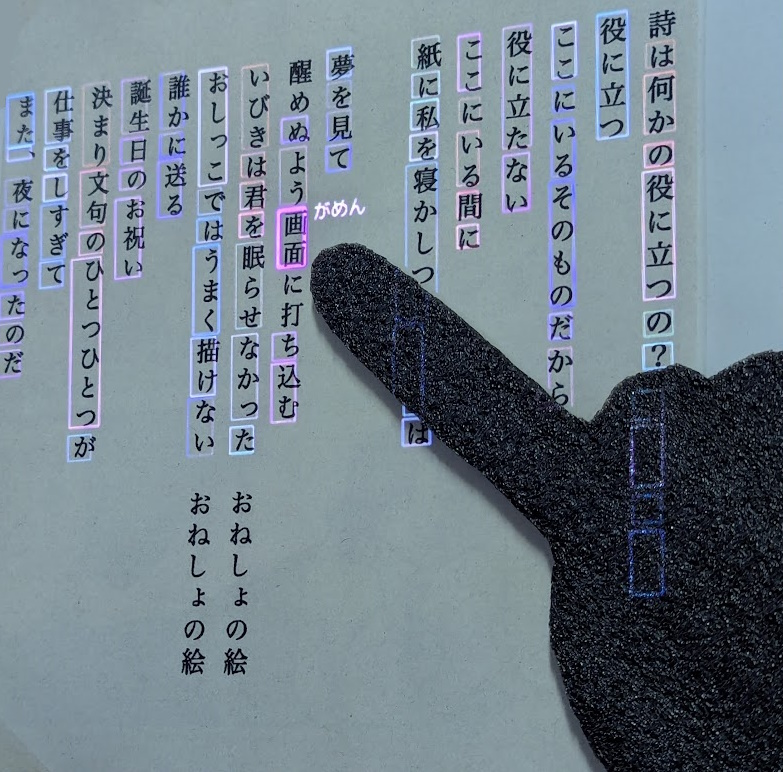
\includegraphics[width=1\hsize]{figure/Gamen-close.jpg}
\caption{The system displays the reading of Japanese Kanji words the user points at.}
\end{figure}

\section{Introduction}

This project seeks to \textbf{enhance language learning}, particularly Japanese, by integrating assistive projections with physical text. Using a camera-projector system, the text and the user’s hand are scanned to enable intuitive interactions. For example, pointing at a section of text allows users to display translations or view the readings of Japanese Kanji, bridging the interactivity of digital tools with the tactile experience of physical books. 

A key motivation for this project is to transform \textbf{physical books into interactive tools} comparable to e-readers while retaining their \textbf{unique advantages}. Physical books offer a tangible and sensory experience that can aid in memory retention \cite{mangen2019comparing}, providing benefits that digital alternatives often lack.


\subsection{Key Features}
The system shall offer two primary functionalities: \textbf{Furigana} display and \textbf{translations}. Furigana, the Hiragana readings above Kanji, can make Kanji easier to read \cite{palmer2012effect} and look up, ensuring correct pronunciation. They can be displayed permanently or triggered by user gestures, such as pointing. For translations, the system displays meanings of words or Kanji in text or symbol form, encouraging active learning. Displaying translations on surfaces like fingernails is also explored to reduce text obstruction, though challenges such as curvature and reflection properties remain.

\subsection{Limitations}
The system has several \textbf{limitations}. It relies on projections, which require a sufficiently dark environment for effective functioning. Increasing projector brightness to address this can result in higher energy consumption and potential health risks. Furthermore, the system depends on continuous power and computationally intensive \textbf{Optical Character Recognition (OCR)} to recognize text. To mitigate this, methods like caching could be employed to reduce computational load. Despite these challenges, this system simplifies interactions and provides unique functionality, offering a new way to interact with and learn from physical texts.

\newpage

\subsection{Physical Setup}

The Physical Setup involves aligning the camera and projector using a mirror to project and capture content on a table with the text medium. A light source can be added to enhance the contrast of the captured image. To minimize reflections, the back of the mirror facing the camera is covered with a black cloth.

\begin{figure}[H] % Use [H] to force the placement here
    \centering
    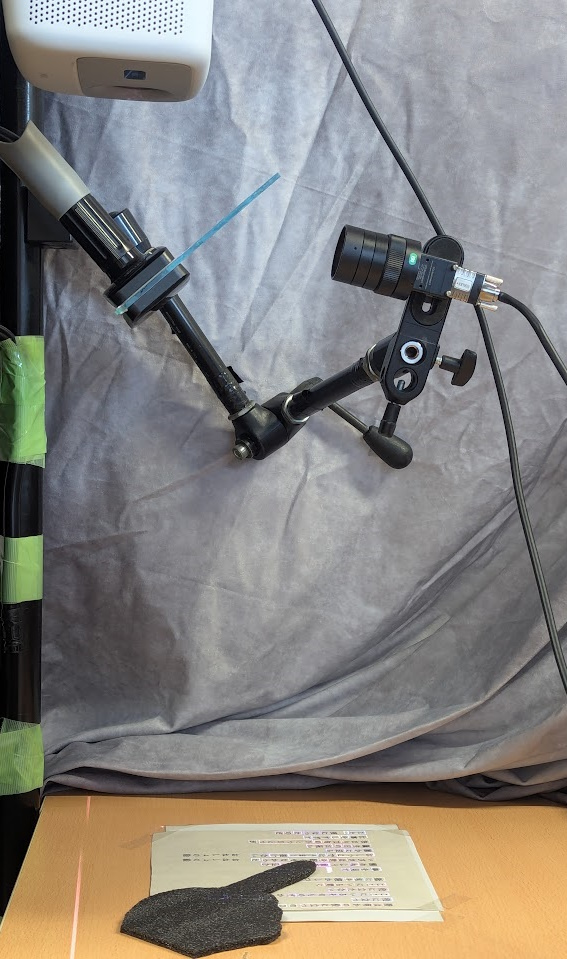
\includegraphics[width=0.7\hsize]{figure/Gamen-total.jpg}
    \caption{The physical setup, including a projector, mirror, camera, table, a Japanese poem, and an artificial black hand for testing.}
\end{figure}

\subsection{System Workflow}

The system workflow comprises several key steps:  

\textbf{1. Fingertip Detection:} The system detects the user’s fingertip and interprets potential gestures for interaction.  

\textbf{2. Text Recognition:} The text is scanned, characters are identified, and their positions are marked with bounding boxes for further processing.  

\textbf{3. Content Generation:} Based on the detected text and gestures, the system generates content for projection, such as translations or Furigana.  

\textbf{4. Projection:} The generated content is projected onto the medium, considering the transformations and alignments of the camera and projector.





\section{Related Work}

\subsection{Related Hardware}

Camera-projector systems for enhancing flat surfaces have been extensively studied since Wellner’s work in 1993. His system demonstrated the recognition of simple gestures, such as touching projected content. Since then, various advancements have been made to improve interaction:

\begin{itemize}
    \item \textbf{LuminAR Desk Lamp (2010):} Linder et al. developed a lamp that could self-adjust and recognize hand gestures for controlling projections \cite{linder2010luminar}.
    \item \textbf{Interactive Tables (2017):} Margetis et al. implemented gesture-based controls for public tables, enabling intuitive navigation of maps \cite{margetis2017interacting}.
    \item \textbf{Augmented Books (2011):} Dachselt et al. introduced a system for annotating physical books using projected tools, though it required special paper for functionality \cite{dachselt2011interacting}.
    \item \textbf{Enhanced Books (2014):} Gebhardt et al. improved on augmented books by eliminating the need for special paper and introducing advanced features for organizing text \cite{gebhardt2014employing}.
    \item \textbf{E-reader Extensions (2012):} Thom et al. designed an e-reader system with a wearable wristband for feedback and hand gestures, maintaining the tactile experience of reading a physical book \cite{thom2012holding}.
\end{itemize}



\begin{figure}[H]
    \centering
    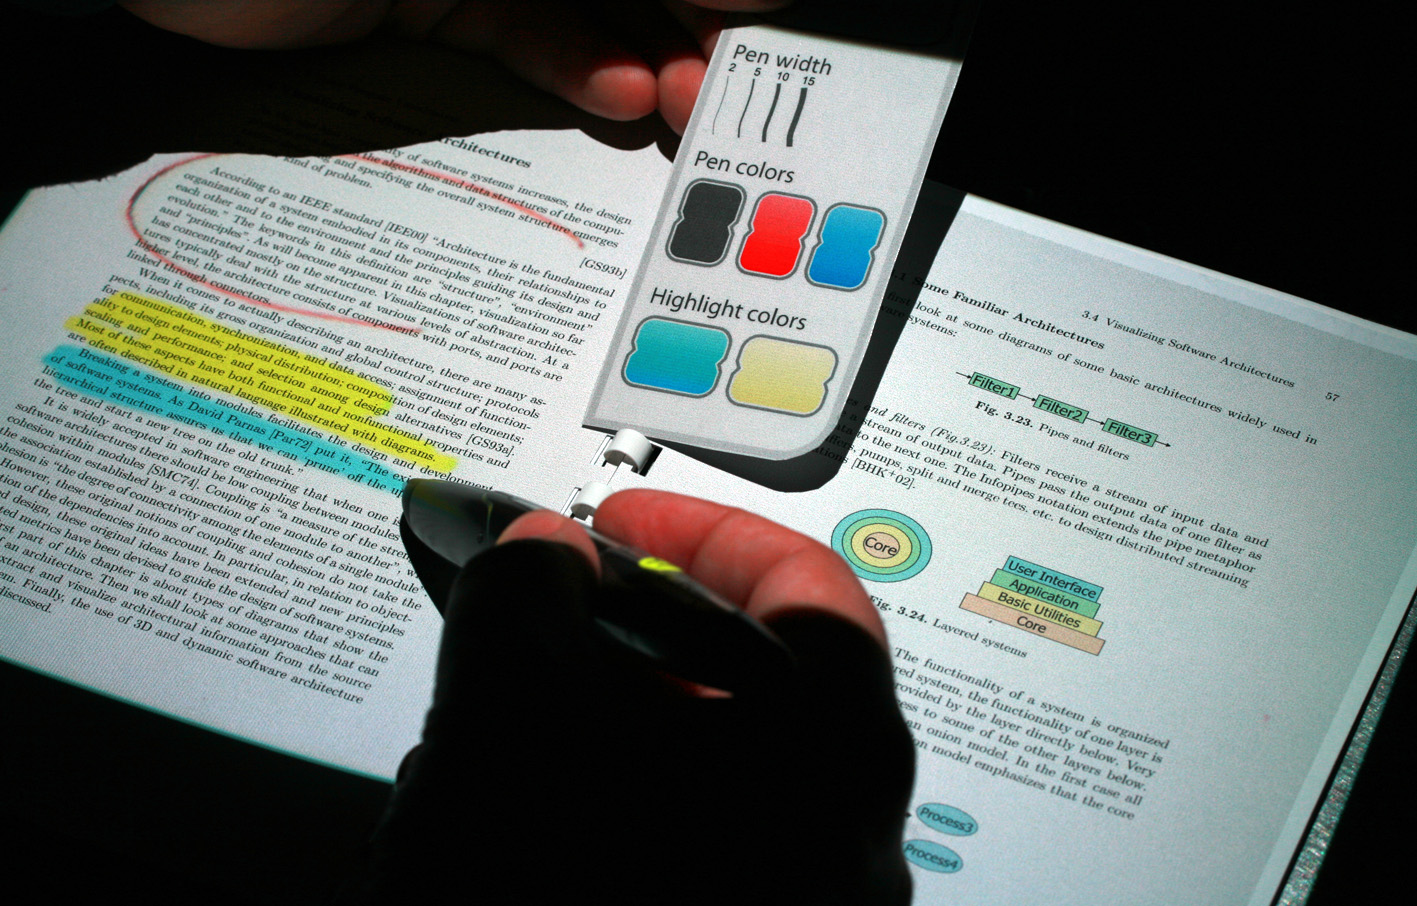
\includegraphics[width=1\linewidth]{figure/related/Interacting-with-books.png}
    \caption{Camera-projection setups for enhancing interaction with physical text have been explored in previous studies, such as Dachselt et al.'s work on augmented books \cite{dachselt2011interacting}.}
\end{figure}

These systems form the foundation for creating a solution that combines advanced interaction with physical texts using simple gestures and projections. Such advancements are particularly relevant for language learning, where engaging with content in real-time can improve accessibility and retention.

\subsection{Related Software}

\textbf{Yomitai}\cite{yomitai} is a web-based tool that displays the readings and meanings of Kanji in uploaded images. It highlights Kanji within the text using color mapping and provides additional information alongside the image.

\textbf{Yomichan}\cite{yomichan} is a browser extension that allows users to hover over text on websites to instantly view readings, definitions, and other relevant details. This system shares similarities with the proposed application but introduces a unique feature: interaction through hand gestures for controlling and engaging with content.

\begin{figure}[H] % Use [H] to force placement
    \centering
    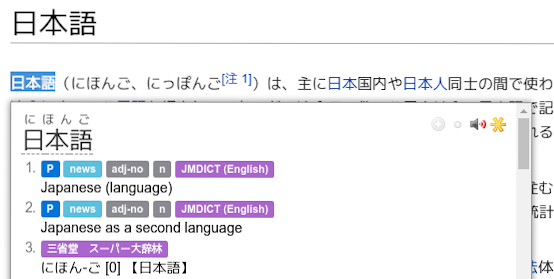
\includegraphics[width=0.9\linewidth]{figure/related/yomichan.png}
    \caption{Yomichan provides readings and definitions for highlighted text directly in the browser.}
    \label{fig:yomichan}
\end{figure}



\section{Fingertip Detection}

Various algorithms have been evaluated for detecting fingertip positions. One challenge is the use of a grayscale camera, which lacks color information to distinguish the hand from the background. Future work plans to address this by switching to an RGB camera.

Detection methods can be broadly categorized into \textbf{machine learning-based} and \textbf{manual detection}. For manual detection, the hand is isolated from the background, and the fingertip is identified. A simple approach that works reasonably well for testing involves finding the highest \textit{y}-coordinate of the hand contour. To avoid misclassifying straight contours from the background, contours with flat edges can be discarded before calculating the highest \textit{y}-coordinate.

To maintain simplicity, stereoscopic or depth cameras were not evaluated, as good results are achievable without them. Additionally, complex methods based on analyzing specific geometric curves were avoided. Future implementations may consider using \textbf{optical flow} for more robust tracking and dynamic hand motion detection.

\begin{figure}[H]
    \centering
    \begin{minipage}{0.48\linewidth}
        \centering
        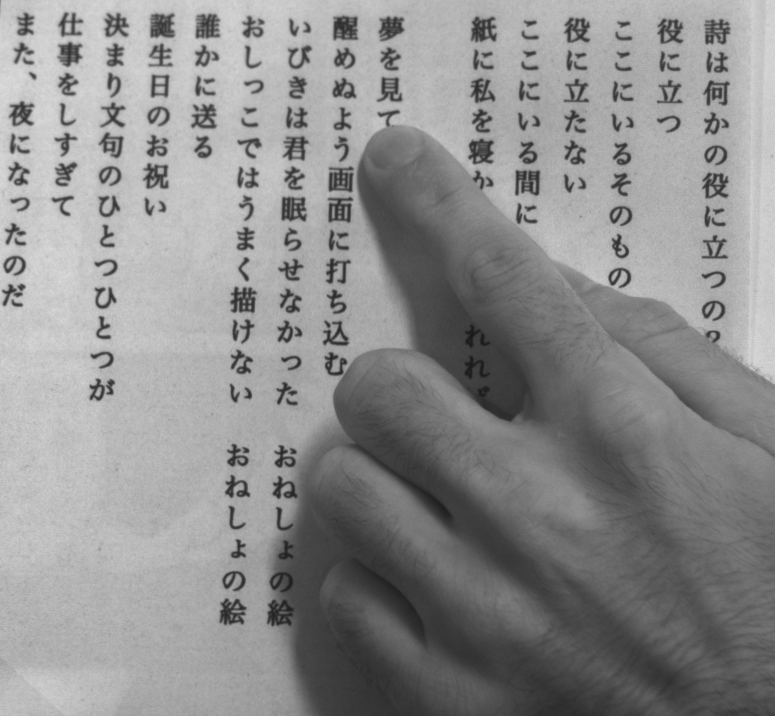
\includegraphics[width=\linewidth]{figure/hand/text.png}
    \end{minipage}
    \hfill
    \begin{minipage}{0.48\linewidth}
        \centering
        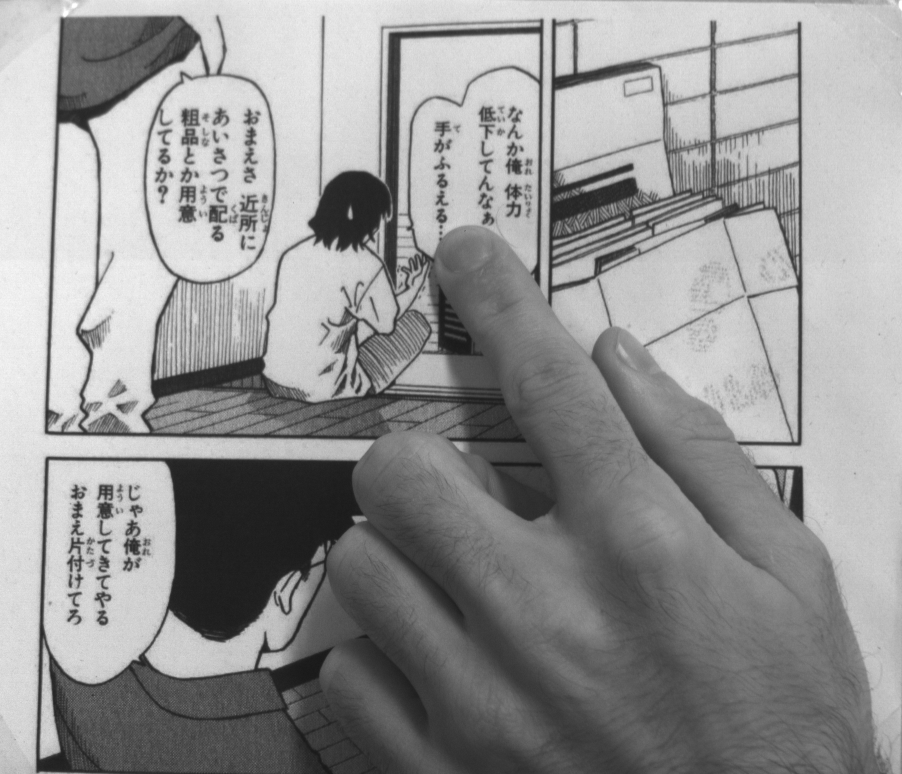
\includegraphics[width=\linewidth]{figure/hand/manga.png}
    \end{minipage}
    \caption{Comparison images for evaluating hand contour segmentation algorithms.}
\end{figure}

\subsection{Dilating}

An initial approach for segmenting the hand involved using \textbf{dilating}, a morphological operation that shrinks black areas and then grows them back to preserve the approximate shape of the hand. This method effectively removes thin text strokes while retaining the hand’s contour.

Under consistent lighting and with sufficient contrast between the hand and the background, this approach delivers good results. However, it struggles when drawings or images are present, as these elements cannot be reliably removed by this method alone. In such cases, combining \textbf{dilating} with an \textbf{edge detection filter} can improve results depending on the specific use case.

\begin{figure}[H]
    \centering
    \begin{minipage}{0.48\linewidth}
        \centering
        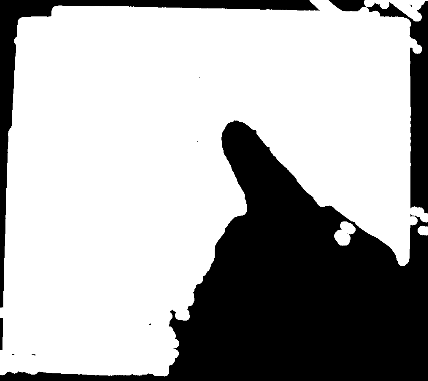
\includegraphics[width=\linewidth]{figure/hand/dilate-text.png}
    \end{minipage}
    \hfill
    \begin{minipage}{0.48\linewidth}
        \centering
        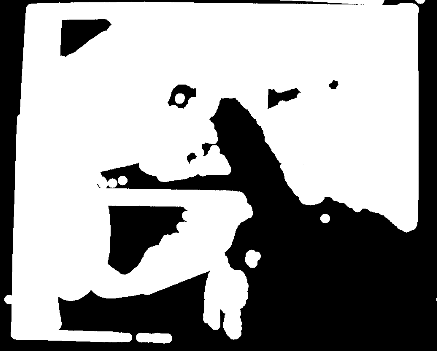
\includegraphics[width=\linewidth]{figure/hand/dilate-manga.png}
    \end{minipage}
    \caption{\textbf{Dilating:} Successfully removes thin text strokes but struggles with complex images.}
\end{figure}

\subsection{Background Subtraction}

Background subtraction involves creating a model of the background and identifying differences compared to a reference image. A key challenge, particularly for grayscale images, is that areas where the hand and background share similar brightness values are not recognized, leading to poor segmentation results.

\subsubsection{Static Background Subtraction}

The simplest approach to background subtraction is generating a \textbf{difference image} under the assumption that the background is static or can be stabilized algorithmically. For flat text media, such as a sheet of paper, \textbf{stabilization} can be achieved using \textbf{feature matching} combined with homographic or affine transformations. This method is effective when the background remains stationary and predictable.

\begin{figure}[H]
    \centering
    \begin{minipage}{0.48\linewidth}
        \centering
        
\includegraphics[width=\linewidth]{figure/hand/difference-text.png}
    \end{minipage}
    \hfill
    \begin{minipage}{0.48\linewidth}
        \centering
        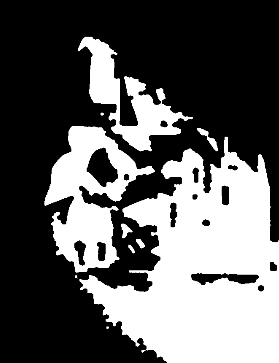
\includegraphics[width=\linewidth]{figure/hand/difference-manga.png}
    \end{minipage}
    \caption{\textbf{Subtraction methods} perform poorly in areas with minimal color changes.}
\end{figure}

\subsubsection{Dynamic Background Subtraction}

For more dynamic environments, tools such as \texttt{cv2.createBackgroundSubtractorKNN()} can be used to create a model that adapts to changing backgrounds. This method dynamically updates the background model to accommodate variations, such as lighting changes or slow movements. However, it struggles with \textbf{very slow or corrective hand movements}, which may not be detected reliably, resulting in incomplete segmentation.

\begin{figure}[H]
    \centering
    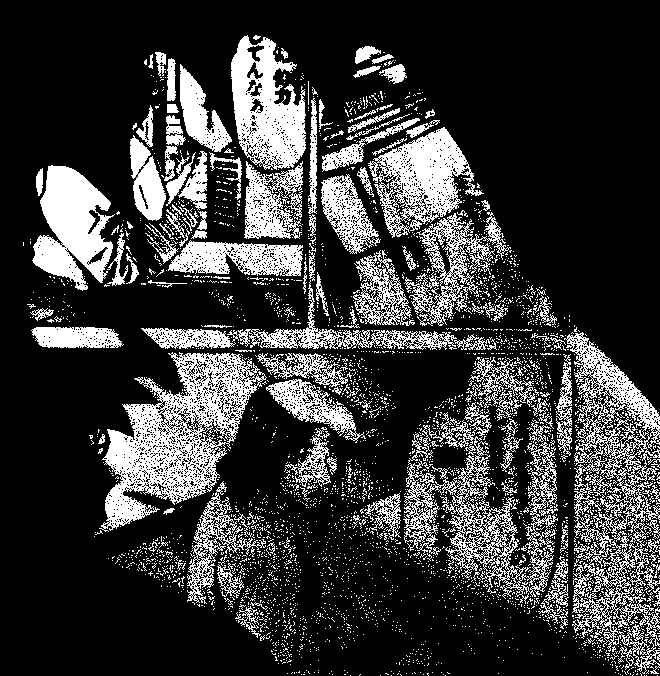
\includegraphics[width=1\linewidth]{figure/hand/movement-manga.png}
    \caption{\textbf{Dynamic subtraction:} Using \texttt{cv2 BackgroundSubtractorKNN} to detect hand movements in dynamic settings.}
\end{figure}


\subsection{Machine Learning}

Machine learning algorithms provide a viable option for directly detecting fingertip positions. However, many pre-trained models are optimized for wide-angle images and struggle to perform well with the narrow field of view used in this system.

\textbf{Mediapipe} \cite{mediapipe} is one such model that requires both the fingers and the wrist to be visible for reliable hand detection. This makes it unsuitable for scenarios where only part of the hand is captured. As shown in the figure below, Mediapipe only recognizes the hand when a sufficiently large portion is visible.

\begin{figure}[H]
    \centering
    \begin{minipage}{0.48\linewidth}
        \centering
        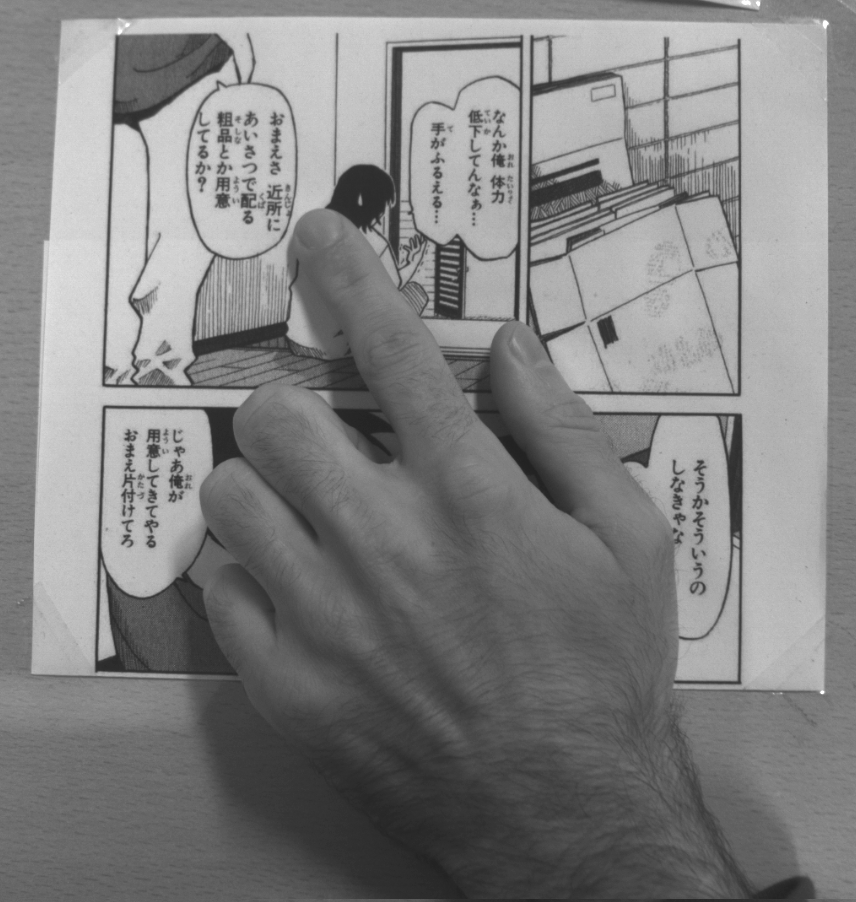
\includegraphics[width=\linewidth]{figure/mediapipe/mediapipe-no.png}
    \end{minipage}
    \hfill
    \begin{minipage}{0.48\linewidth}
        \centering
        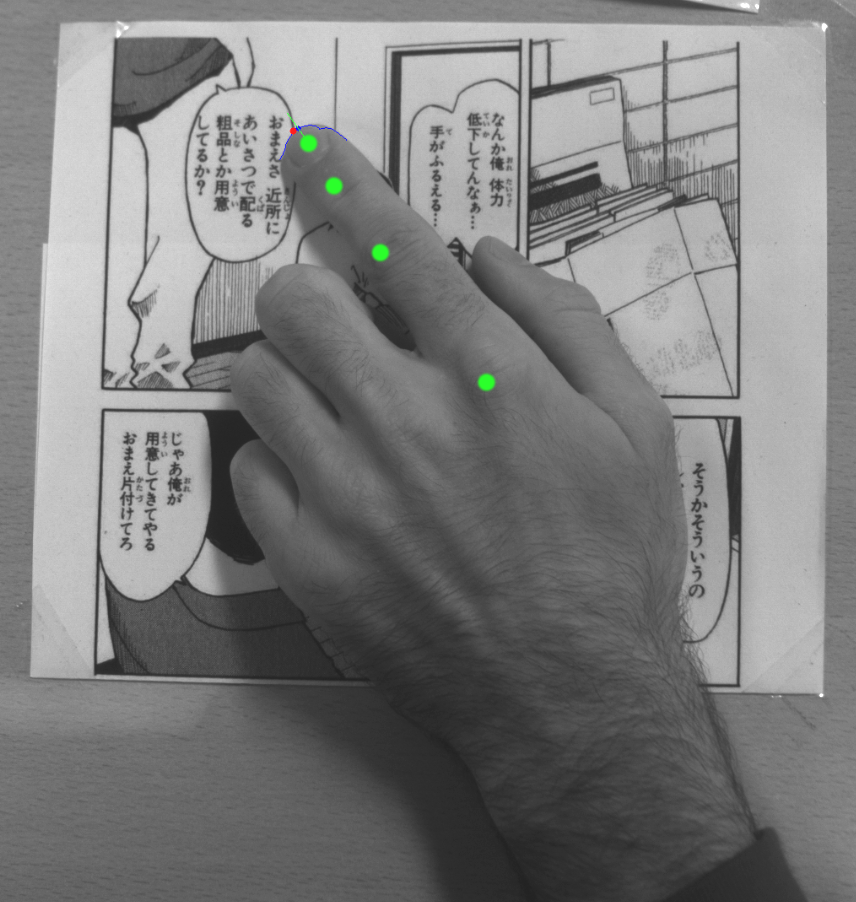
\includegraphics[width=\linewidth]{figure/mediapipe/mediapipe-yes.png}
    \end{minipage}
    \caption{\textbf{Mediapipe:} The hand is only recognized on the right side when enough of it is visible in the frame.}
\end{figure}

\textbf{Unified-Gesture-and-Fingertip-Detection} \cite{unified_gesture}, another model, requires color images to function. It suffers from significant accuracy issues when the hand is not fully visible within the frame, making it unreliable for partial hand detection scenarios.

\begin{figure}[H]
    \centering
    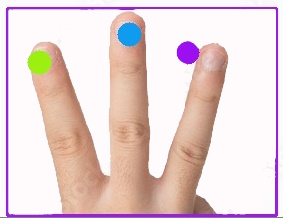
\includegraphics[width=0.9\hsize]{figure/unified-fingertip-detection.jpg}
    \caption{\textbf{Unified-Gesture-and-Fingertip-Detection:} The model performs poorly when parts of the hand are cutoff.}
\end{figure}

Considering these limitations, training a \textbf{custom machine learning model} tailored to the specific requirements of this system shall be explored in the future. Custom training can provide a significant advantage, as machine learning algorithms typically achieve the highest accuracy when adapted to their target scenarios.


\section{Text Recognition}

Text Recognition or Optical Character Recognition (OCR) is a critical component for detecting characters in captured images. Free OCR tools such as \texttt{TesseractOCR} \cite{tesseract}, \texttt{PaddleOCR} \cite{paddleocr}, and \texttt{MangaOCR} \cite{mangaocr} are widely available, alongside online services like \texttt{Google Vision} \cite{google_cloud_vision_ocr}, which provide free functionality within a limited usage quota.

The primary use cases for this system include recognizing plain black text on white backgrounds and detecting text in speech bubbles within manga, where backgrounds are often non-white. A suitable OCR library must identify individual words or characters along with their bounding boxes to enable user interaction.

\subsection{Free OCR Libraries}

\textbf{TesseractOCR} is capable of recognizing individual characters, but it struggles with accurately determining bounding boxes. Symbols are often misaligned with their corresponding bounding boxes, leading to errors in interpretation.

\begin{figure}[H]
    \centering
    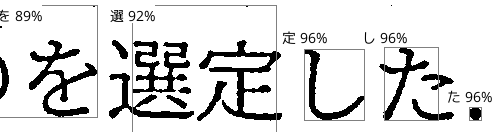
\includegraphics[width=1\hsize]{figure/Tesseract-Fail.png}
    \caption{\textbf{TesseractOCR:} Bounding boxes are partially incorrect and shifted, reducing accuracy.}
\end{figure}

\textbf{PaddleOCR} reliably detects text on white backgrounds but is limited to recognizing text sections separated by spaces. Extensive parameter tuning did not resolve its inability to provide precise character-level bounding boxes.

\textbf{MangaOCR} is specialized for recognizing text in manga. However, it only outputs plain strings without bounding boxes, making it unsuitable for applications requiring precise spatial alignment.

Both Tesseract and PaddleOCR perform poorly on manga text, with only a fraction of the text accurately detected. Despite their general-purpose capabilities, these tools lack the robustness needed for the specific requirements of this system.

\subsection{Manual Segmentation of Kanji}

Printed Kanji typically have consistent width and height, making segmentation theoretically possible by collecting bounding boxes for contours and merging them with an intelligent algorithm. The segmented characters can then be recognized individually using a free OCR engine. However, challenges arise with characters like \textit{い}, which include internal whitespace that may interfere with the segmentation process. This approach could also be combined with bounding boxes obtained from OCR engines. Nonetheless, it was not pursued further in favor of a more robust solution.

\begin{figure}[H]
    \centering
    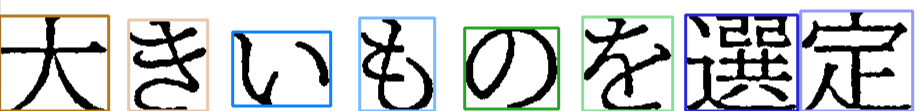
\includegraphics[width=1\hsize]{figure/ocr/manual-character-segmentation.png}
    \caption{\textbf{Manual Segmentation:} Kanji segmentation using merged bounding boxes.}
\end{figure}

\subsection{Google Vision}

The \texttt{Google Vision} web service offers reliable OCR functionality out of the box. It hierarchically organizes text into letters, words, and sections, requiring minimal preprocessing. While it generally performs well, complex Kanji with low resolution may present challenges. Future work aims to address this limitation through artificial upscaling and pre-filtering techniques.

\begin{figure}[H]
    \centering
    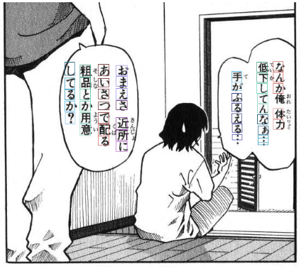
\includegraphics[width=1\hsize]{figure/ocr/GoogleOCR-crop.png}
    \caption{\textbf{Google Vision OCR:} Applied to a manga image, producing near-perfect results (Furigana excluded due to size).}
\end{figure}

The main limitation of \texttt{Google Vision} is its free usage cap of 1,000 queries per month. This issue can be mitigated by saving query results using Python's \texttt{pickle} library for reuse on subsequent system starts. To ensure this approach works, the text must remain in the same position. This can be achieved through physical fixation of the medium and runtime image stabilization, as discussed in the \textit{Background Subtraction} section.
 
 \newpage
 
\section{Content Generation}

Currently, the system focuses on two primary functionalities: drawing \textbf{bounding boxes} around characters and displaying \textbf{Furigana} above them. These features have been evaluated as initial steps toward enabling interactive and dynamic content projection.


\begin{figure}[H] % Use [H] to force placement
\centering
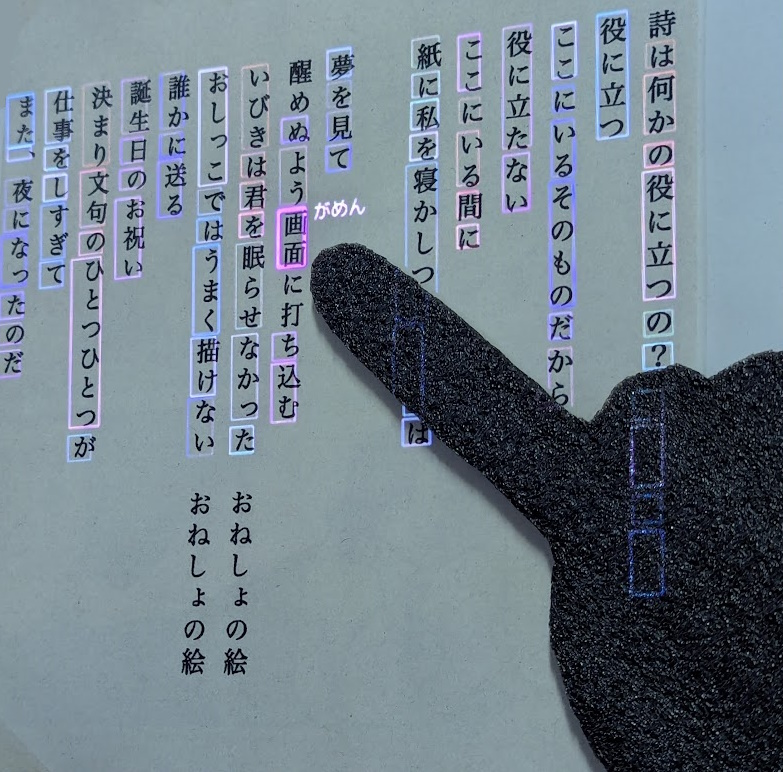
\includegraphics[width=1\hsize]{figure/Gamen-close.jpg}
\caption{The system displays the reading of Japanese Kanji words the user points at.}
\end{figure}


\section{Projection}

For the test setup, a \textbf{JMGO N1 projector} with 4K resolution is utilized. The projector and camera are optically aligned to work with a flat text surface. Calibration is achieved through a \textbf{perspective transform}, which aligns the projection with the captured image. The transformation matrix is computed by solving a system of equations based on four corresponding points between the recorded camera image and the projection image. This approach ensures precise alignment, enabling accurate overlay of projected content onto the physical medium.




%FIG~\ref{fig:System}
%FOOTNOTE~\footnote{https://uiuxtrend.com/pssuq-post-study-system-usability-questionnaire/}{}

%\renewcommand{\theenumi}{\Roman{enumi}}
%\begin{enumerate}
%    \item ITEM 1
%    \item ITEM 2
%    \begin{itemize}
%        \item ITEM 2.1
%        \item ITEM 2.2
%    \end{itemize}
%\end{enumerate}

\bibliographystyle{ipsjunsrt}
\newpage
\bibliography{bibliography}

\end{document}
